\documentclass[14pt,a5paper,twoside]{book}
\usepackage{anysize}
\marginsize{2cm}{2cm}{2cm}{2cm}

%Nastaví kódování na UTF8
\usepackage[utf8]{inputenc}
\usepackage[T1]{fontenc}

%Nastavuje velikost vertikální mezery mezi odstavci
\setlength{\parskip}{0.2ex plus 0.1ex minus 0.1ex}

\usepackage[cc]{titlepic}
\usepackage{graphicx}
\usepackage{fancyhdr}
\usepackage{setspace}

\renewcommand{\rmdefault}{ptm}

% Redefine plain page style
\fancypagestyle{plain}{
\fancyhf{}
\renewcommand{\headrulewidth}{0pt}
\fancyfoot[LE,RO]{\thepage}
}

% Redefine nic page style
\fancypagestyle{nic}{
\fancyhf{}
\renewcommand{\headrulewidth}{0pt}
\renewcommand{\footrulewidth}{0pt}
\fancyfoot[LE,RO]{}
}

\renewcommand{\chaptermark}[1]{\markboth{#1}{}}
\renewcommand{\sectionmark}[1]{\markright{#1}{}}

\renewcommand{\footrulewidth}{0.4pt}
\fancyfoot[CO,CE]{www.zonglovani.info}
\fancyfoot[RO, LE] {\thepage}

\usepackage{wrapfig}
\usepackage{floatflt}

\parindent=1.2em
\usepackage[czech]{babel}
\usepackage{indentfirst}


% vypnutí číslování nadpisů v textu
%\setcounter{secnumdepth}{-1}

\usepackage[pdftex,colorlinks=true,linkcolor=black,bookmarks=true,unicode,linktocpage=false,pdfdisplaydoctitle=true,bookmarksopenlevel=1]{hyperref}
\usepackage[bookmarks=true]{hyperref}
\hypersetup{
pdfauthor = {Petr Kletečka},
pdftitle = {Žonglérův slabikář},
pdfsubject = {Žonglování},
pdfkeywords = {žonglování, míčky, kruhy, kužely},
pdfcreator = {www.zonglovani.info},
pdfproducer = {www.zonglovani.info}
}
\begin{document}
%\raggedbottom
\frontmatter
\setlength{\parindent}{0pt}

\newcommand{\nbtitlestretch}{\spaceskip0.6em}
\setlength\fboxsep{0pt}
\setlength\fboxrule{0.5pt}
\begin{titlepage}
\pdfbookmark[0]{Obálka}{obalka}
\begin{center}
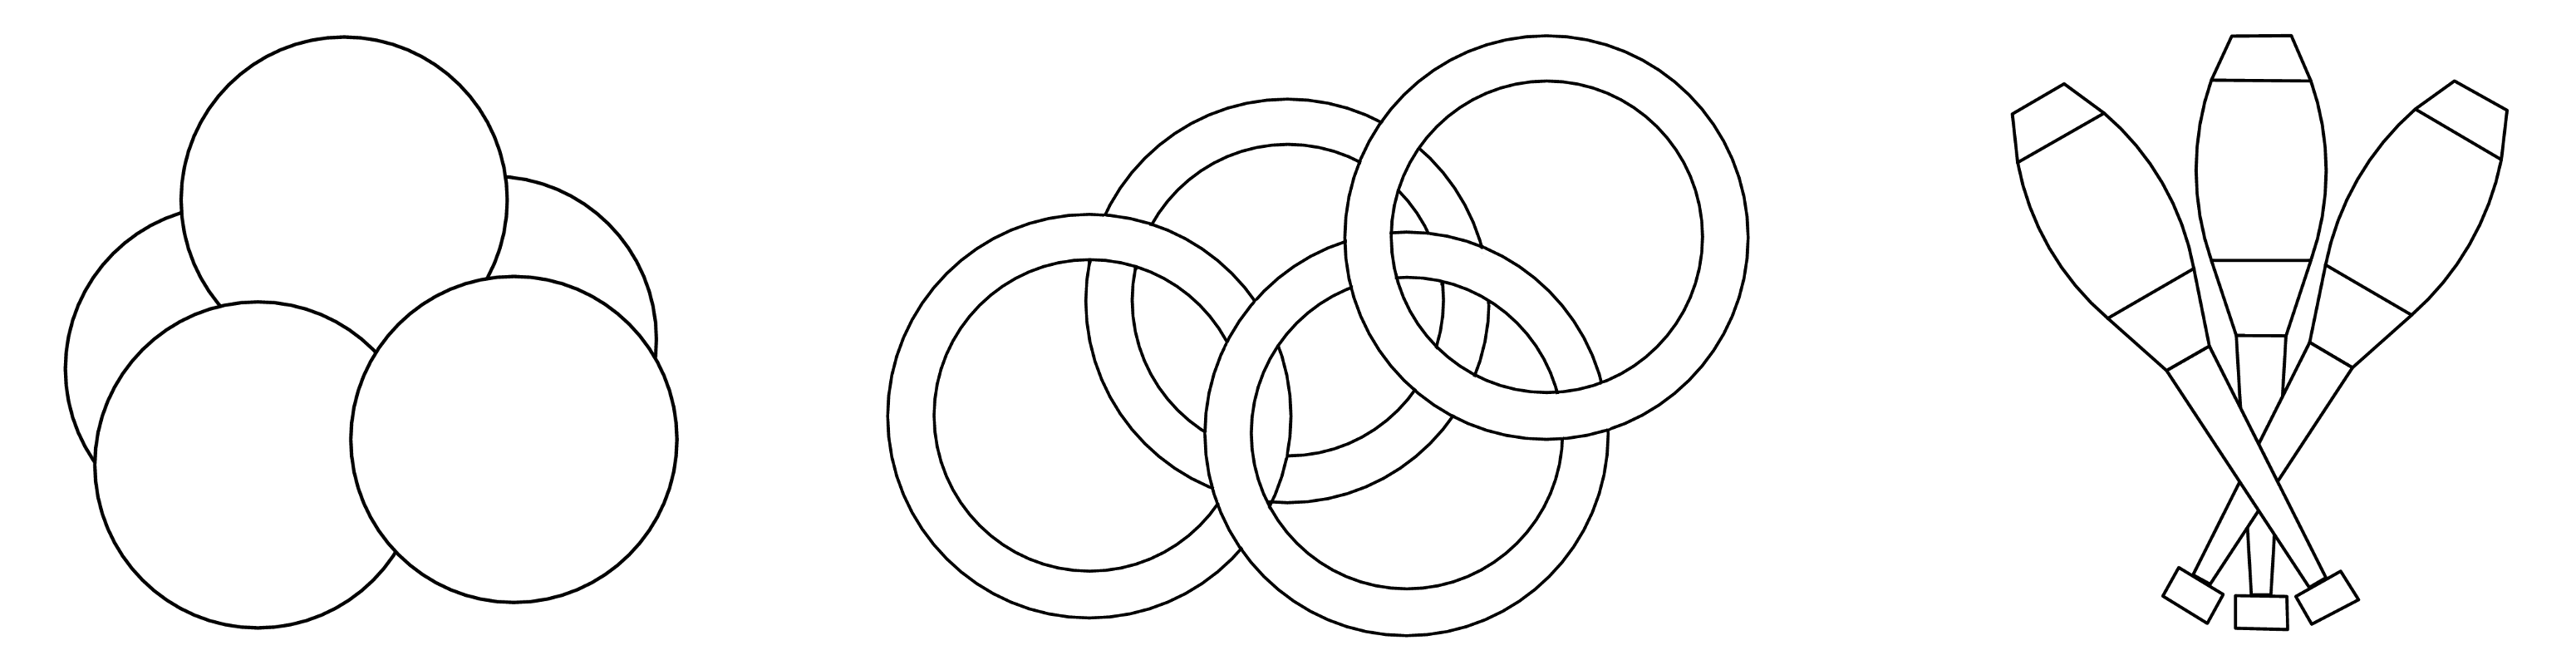
\includegraphics[width=1\textwidth]{obrazky/titleimg.png}
\\[.5cm]

\includegraphics[width=1\textwidth]{obrazky/nadpis.png}
\\[.5cm]
\Large Petr Kletečka
\\[5cm]
www.zonglovani.info
\end{center}
\end{titlepage}

\thispagestyle{nic}
\cleardoublepage
\setcounter{tocdepth}{1}
\pagenumbering{Roman}
\pdfbookmark[0]{Obsah}{obsah}
\tableofcontents{}

\onehalfspacing

\mainmatter
\pagestyle{fancy}
\renewcommand{\arraystretch}{1.1}
\chapter{Tři míčky}

\include{tri-micky}

\chapter{Čtyři míčky}

\include{ctyri-micky}

\chapter{Pět míčků}

\include{pet-micku}

\chapter{Kruhy}

\include{kruhy}

\chapter{Kužely}

\include{kuzely}

\chapter{Passing s kužely}

\include{passing}

\chapter{Doslov}
\section{Poděkování}
Ke vzniku této knihy přispěli: Jitka, Martin, Renáta, Matěj, Olii, Pavel, Eva, Lucka, Vojta, Jana, Ondřej, Mižu, Standa, Vláďa, Adéla, Dáša, Eliška, Dan, Zbyněk, Jirka, Tomáš, Karolína, Cecilka, Hanka, Mirek a další.
\section{Licence}

\includegraphics[width=3cm]{obrazky/cc-by-nd.png}\\
Tento dokument je volně šířitelný pod licencí Creative Commons BY-ND.
Můžeš jej šířit a používat pro komerční i nekomerční účely, musí však být uveden autor a dokument nelze měnit.
\section{Aktualizace}
Nové verze najdeš na stránce www.zonglovani.info.

Tato verze VERSION vznikla \today.
\end{document}
